
\documentclass[11pt]{article}

\usepackage{graphicx}
\usepackage{booktabs}
\usepackage{longtable}
\usepackage{float}
\usepackage{geometry}

\geometry{margin=2.5cm}

\title{Gendered Continuation Analysis}
\date{\today}

\begin{document}

\maketitle

\section{Model Fit}

\begin{tabular}{lrrrrr}
\toprule
Model & AIC & BIC & R2m & R2c & ResidualVariance \\
\midrule
Qwen_Qwen3-4B-Base & 7355.178 & 7648.130 & 0.021 & 0.902 & 0.167 \\
allenai_Olmo-3-1025-7B & 6969.468 & 7255.608 & 0.030 & 0.909 & 0.158 \\
google_gemma-3-4b-pt & 4523.552 & 4809.692 & 0.031 & 0.947 & 0.110 \\
gpt2 & 2096.731 & 2382.870 & 0.019 & 0.905 & 0.076 \\
mistralai_Mistral-7B-v0.3 & 5524.240 & 5810.379 & 0.030 & 0.920 & 0.128 \\
\bottomrule
\end{tabular}


\begin{figure}[H]
\centering

\includegraphics[width=.8\textwidth]{figures/r2_comparison.png}
\caption{Marginal and conditional $R^2$.}
\end{figure}

\begin{figure}[H]
\centering

\includegraphics[width=.8\textwidth]{figures/aic_comparison.png}
\caption{Best-model AIC values.}
\end{figure}

\section{Random Effects}

\begin{tabular}{lrrrr}
\toprule
Model & Semantic role & Syntactic role & Valence & Dominance \\
\midrule
Qwen_Qwen3-4B-Base & 0.0165 & 0.0728 & 0.0045 & 0.0083 \\
allenai_Olmo-3-1025-7B & 0.0019 & 0.0291 & 0.0147 & 0.0132 \\
google_gemma-3-4b-pt & 0.0057 & 0.0183 & 0.0045 & 0.0027 \\
gpt2 & 0.0048 & 0.0298 & 0.0034 & 0.0043 \\
mistralai_Mistral-7B-v0.3 & 0.0037 & 0.0059 & 0.0108 & 0.0049 \\
\bottomrule
\end{tabular}


\begin{figure}[H]
\centering

\includegraphics[width=.9\textwidth]{figures/variance_decomposition.png}
\caption{Random-slope variance decomposition.}
\end{figure}

\section{Profession-Level Structure}

\begin{figure}[H]
\centering
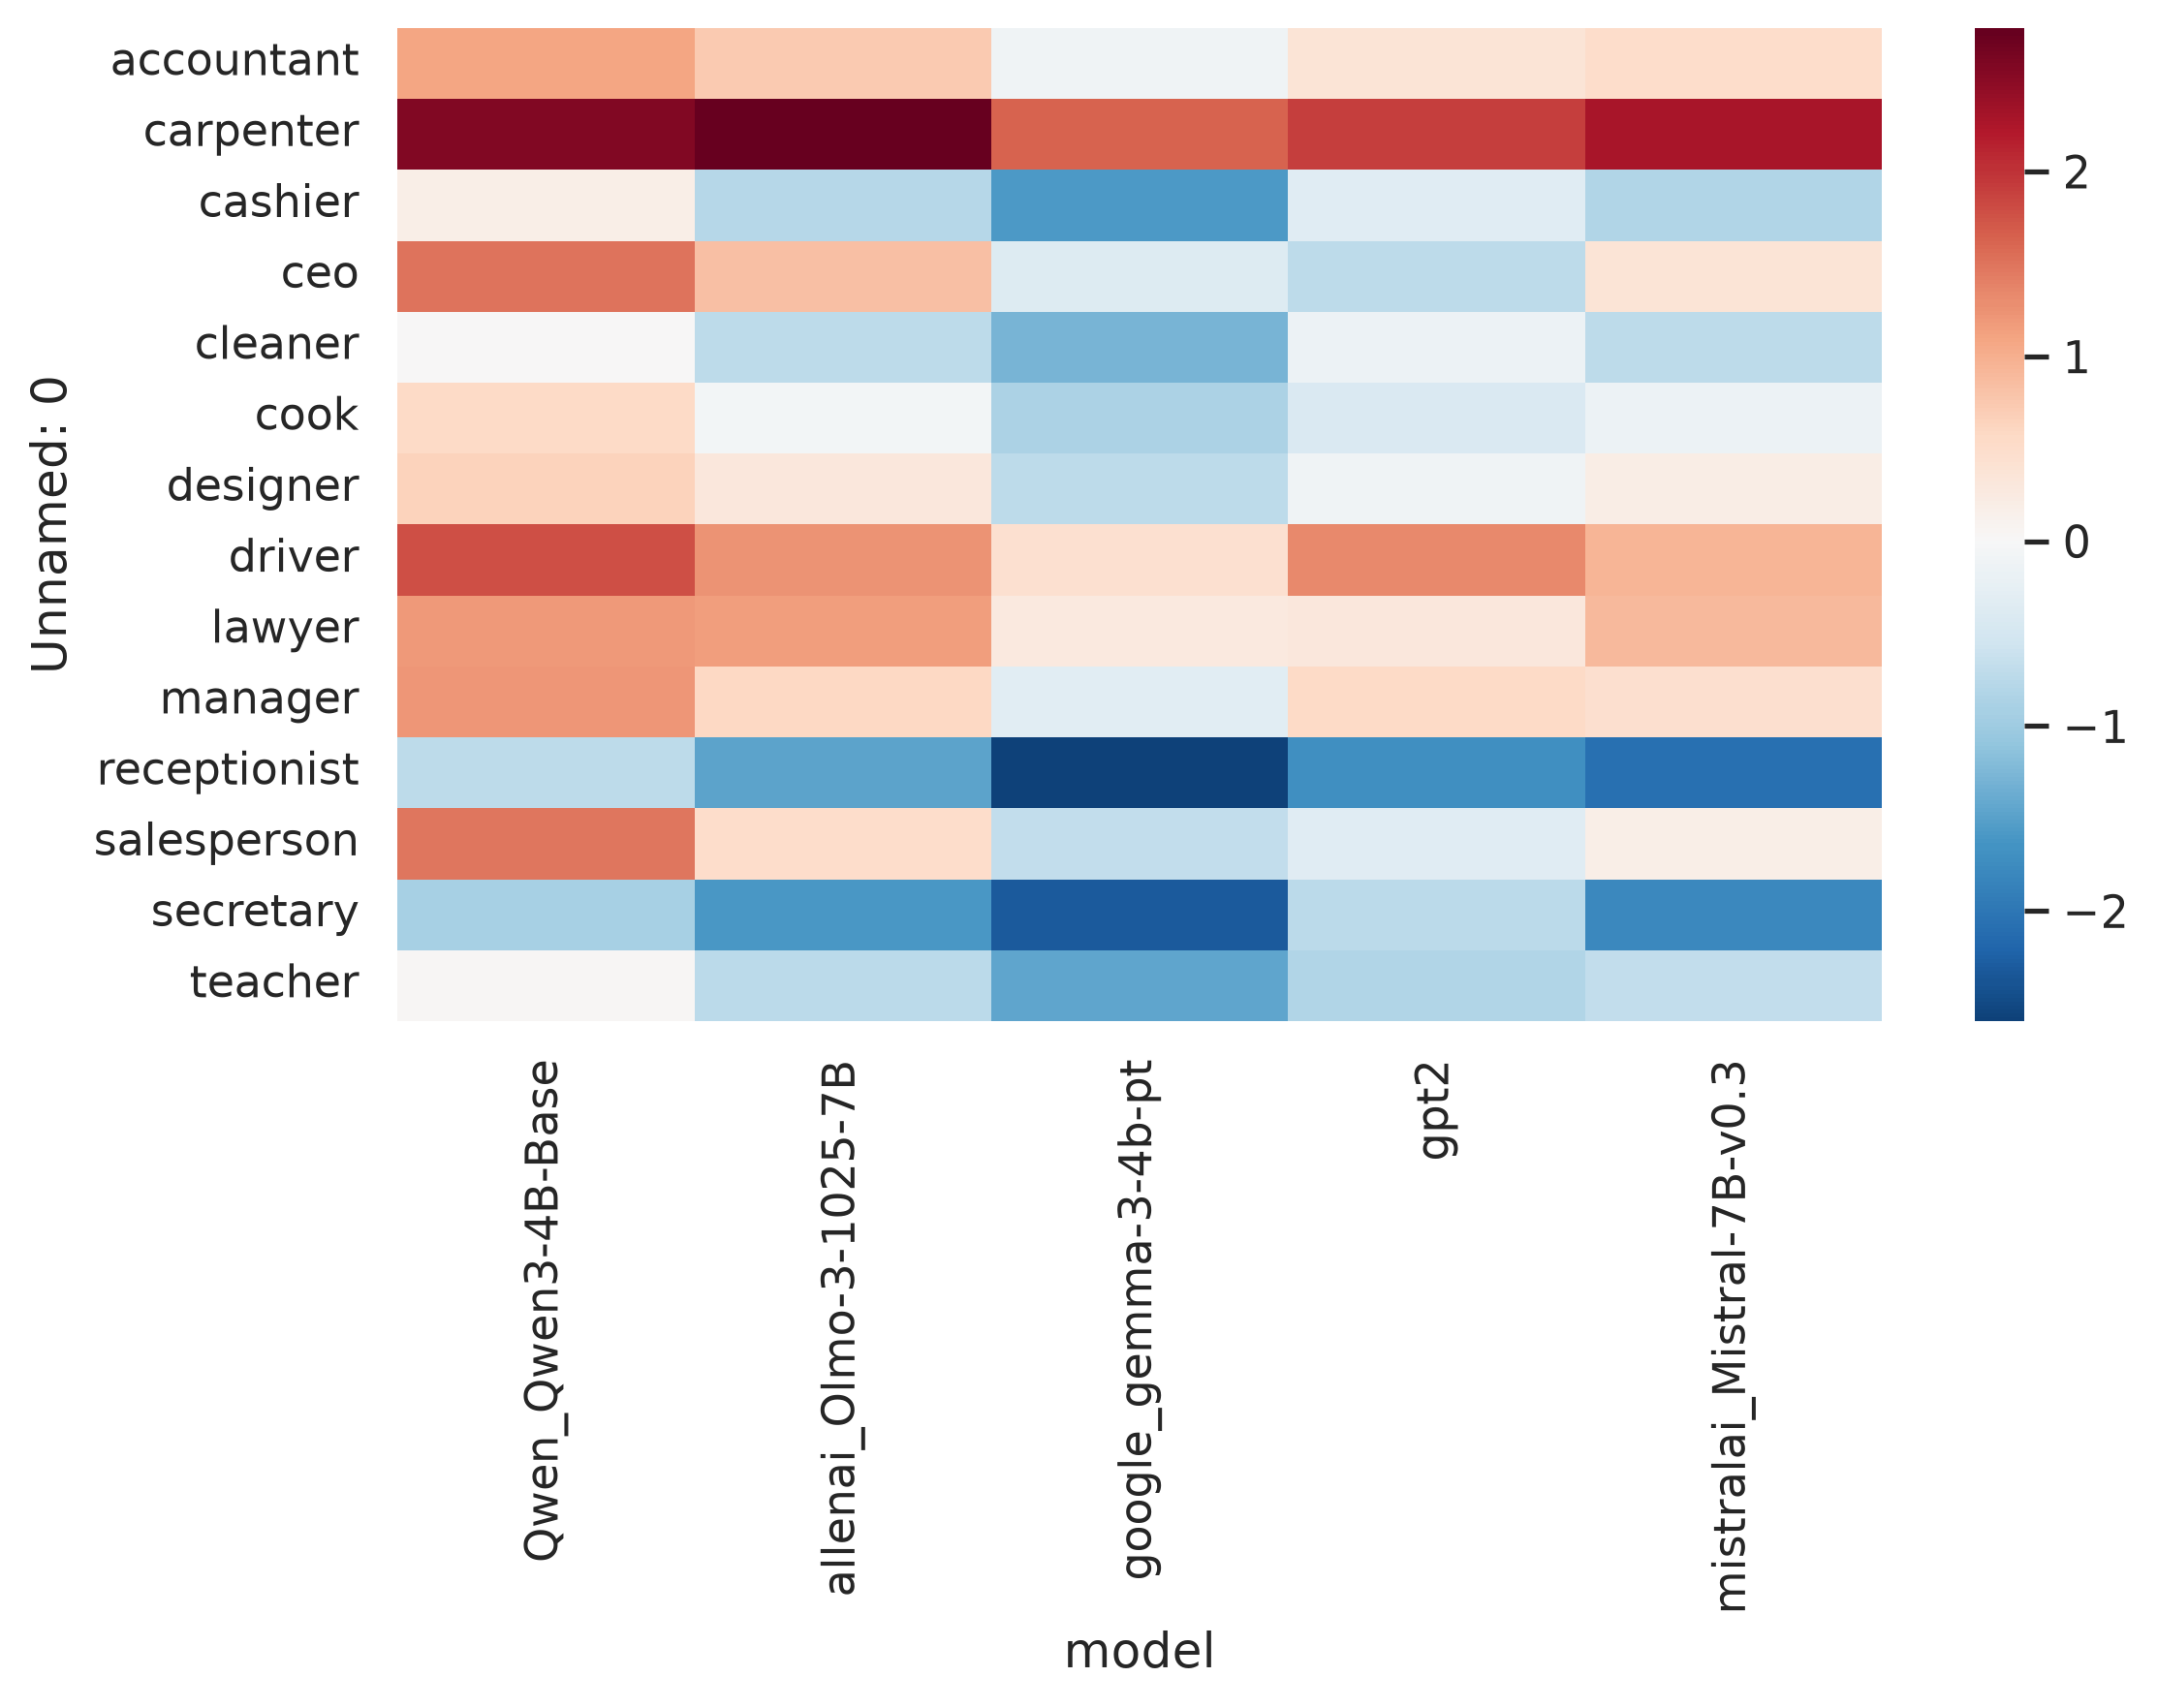
\includegraphics[width=.9\textwidth]{figures/profession_intercepts_heatmap.png}
\caption{Profession intercepts.}
\end{figure}

\begin{figure}[H]
\centering
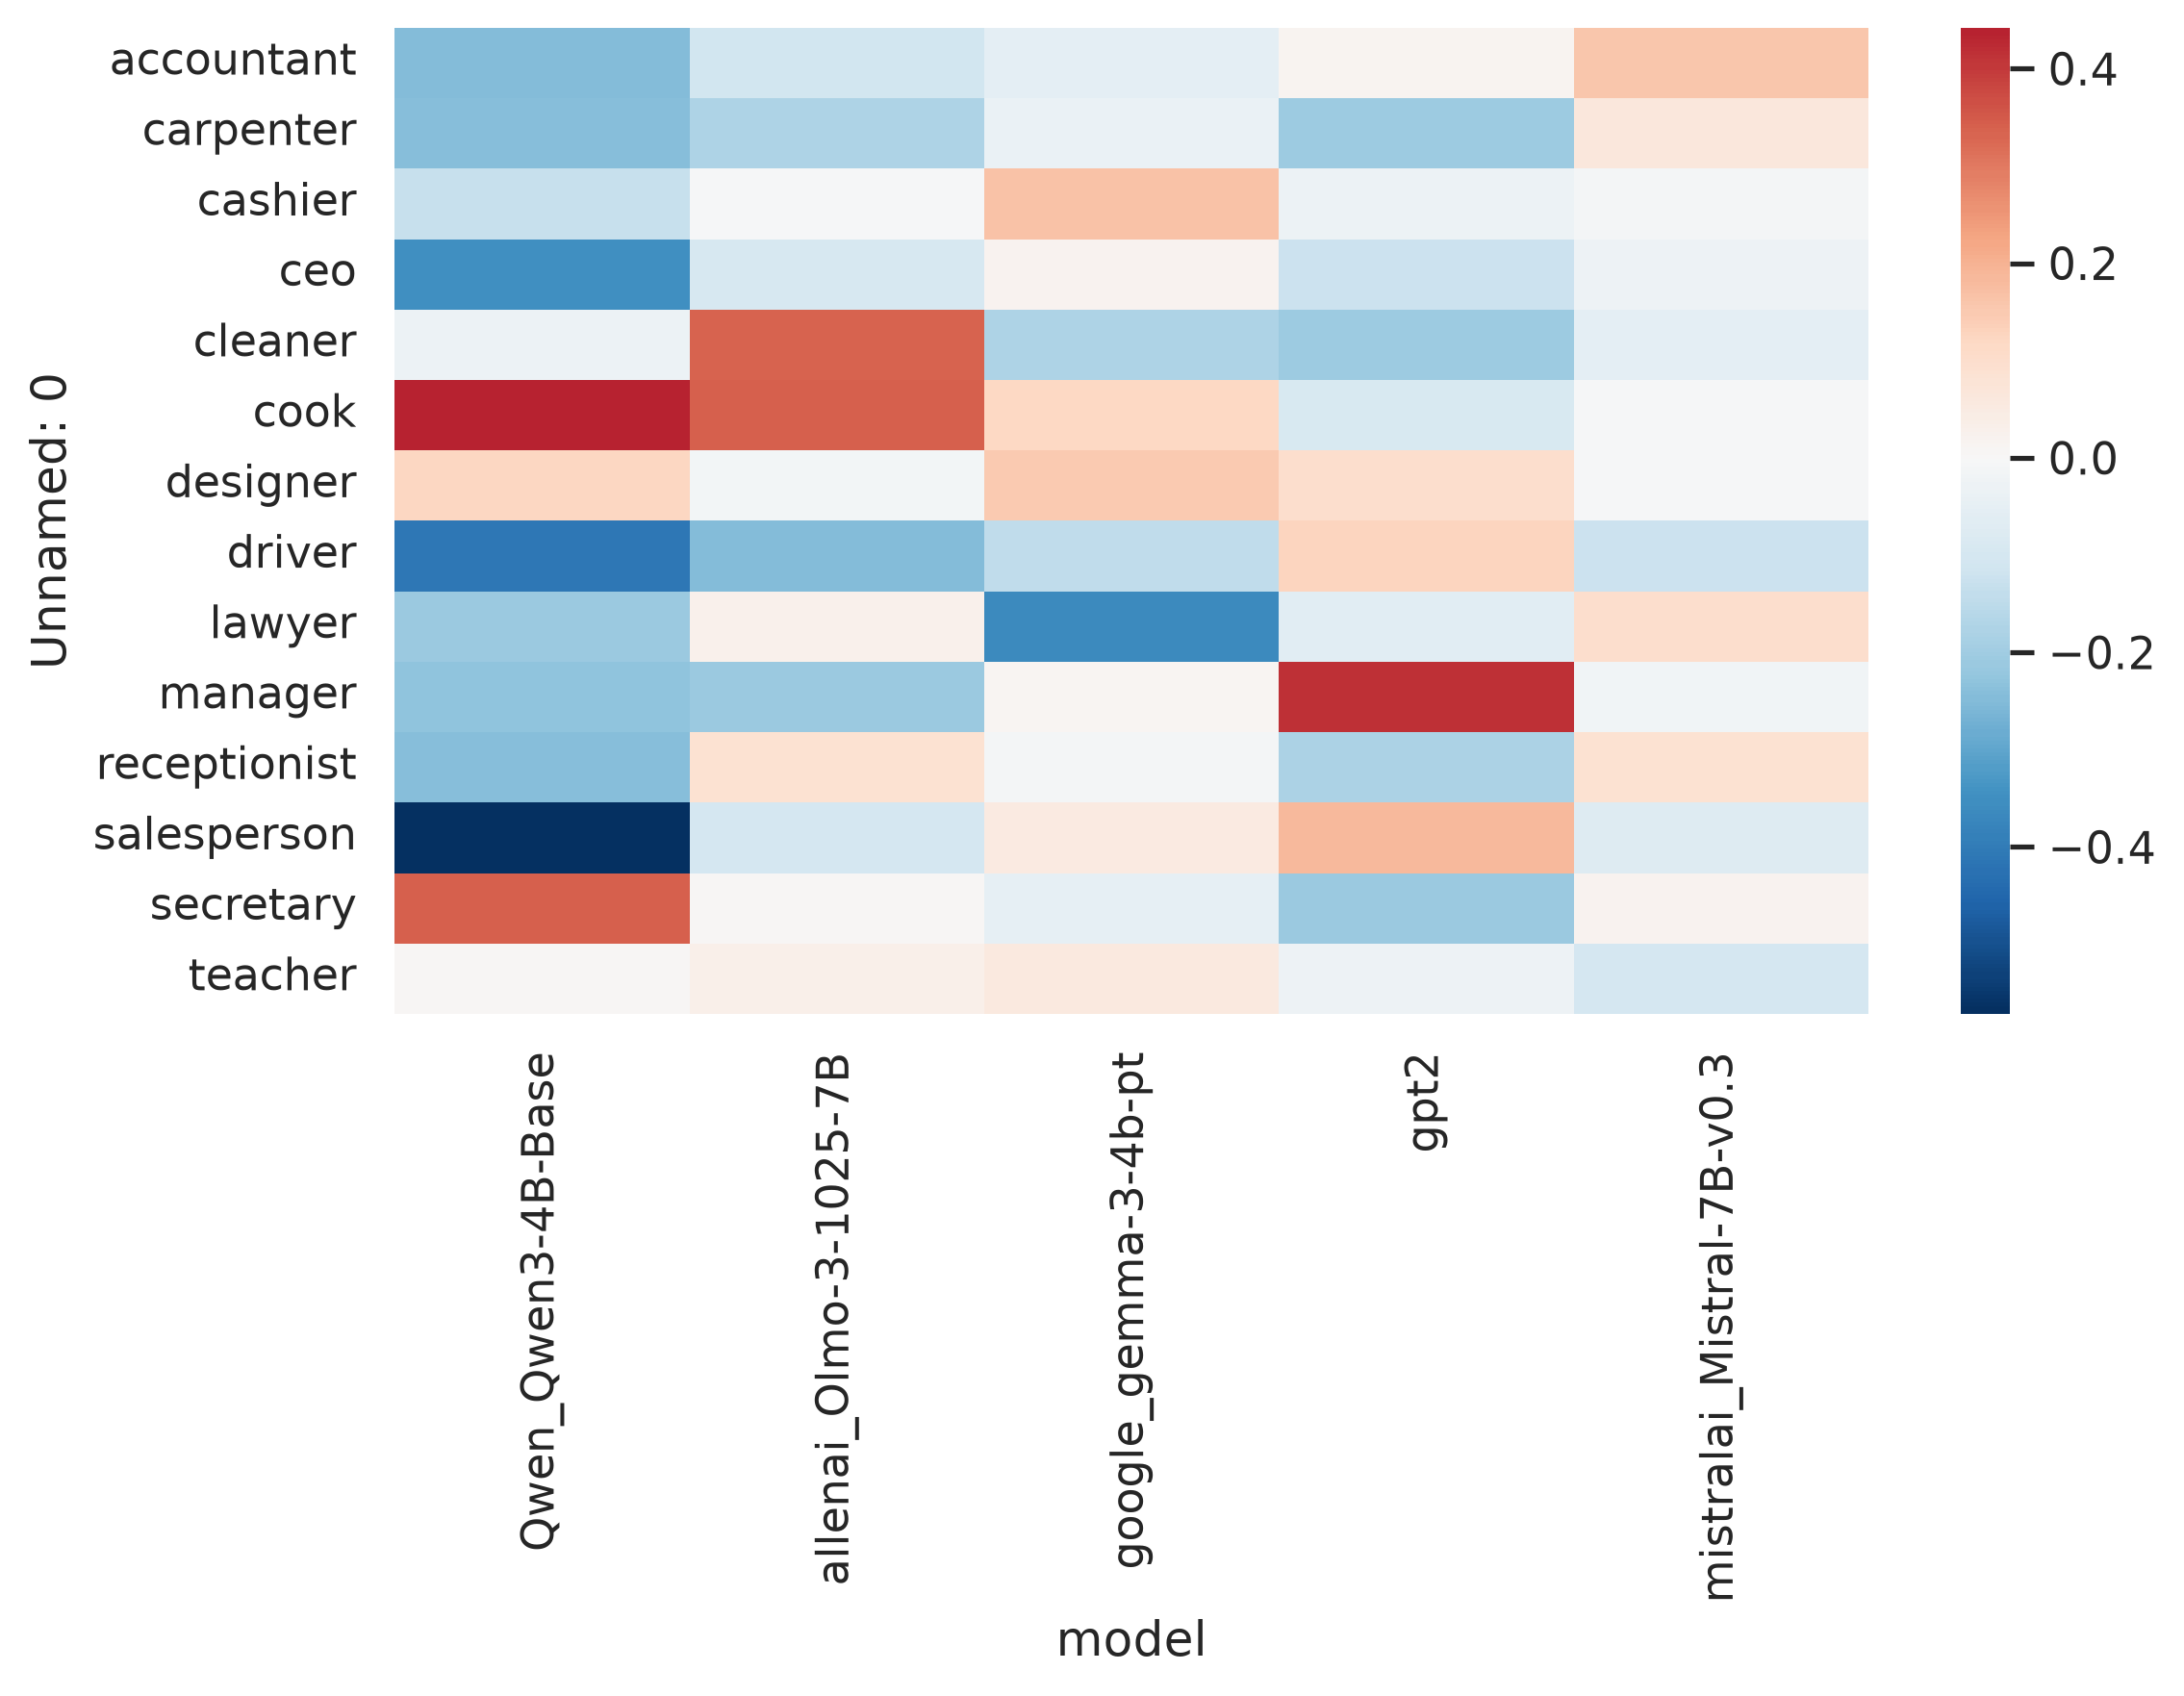
\includegraphics[width=.9\textwidth]{figures/profession_syntactic_role_heatmap.png}
\caption{Syntactic-role random effects.}
\end{figure}

\begin{figure}[H]
\centering
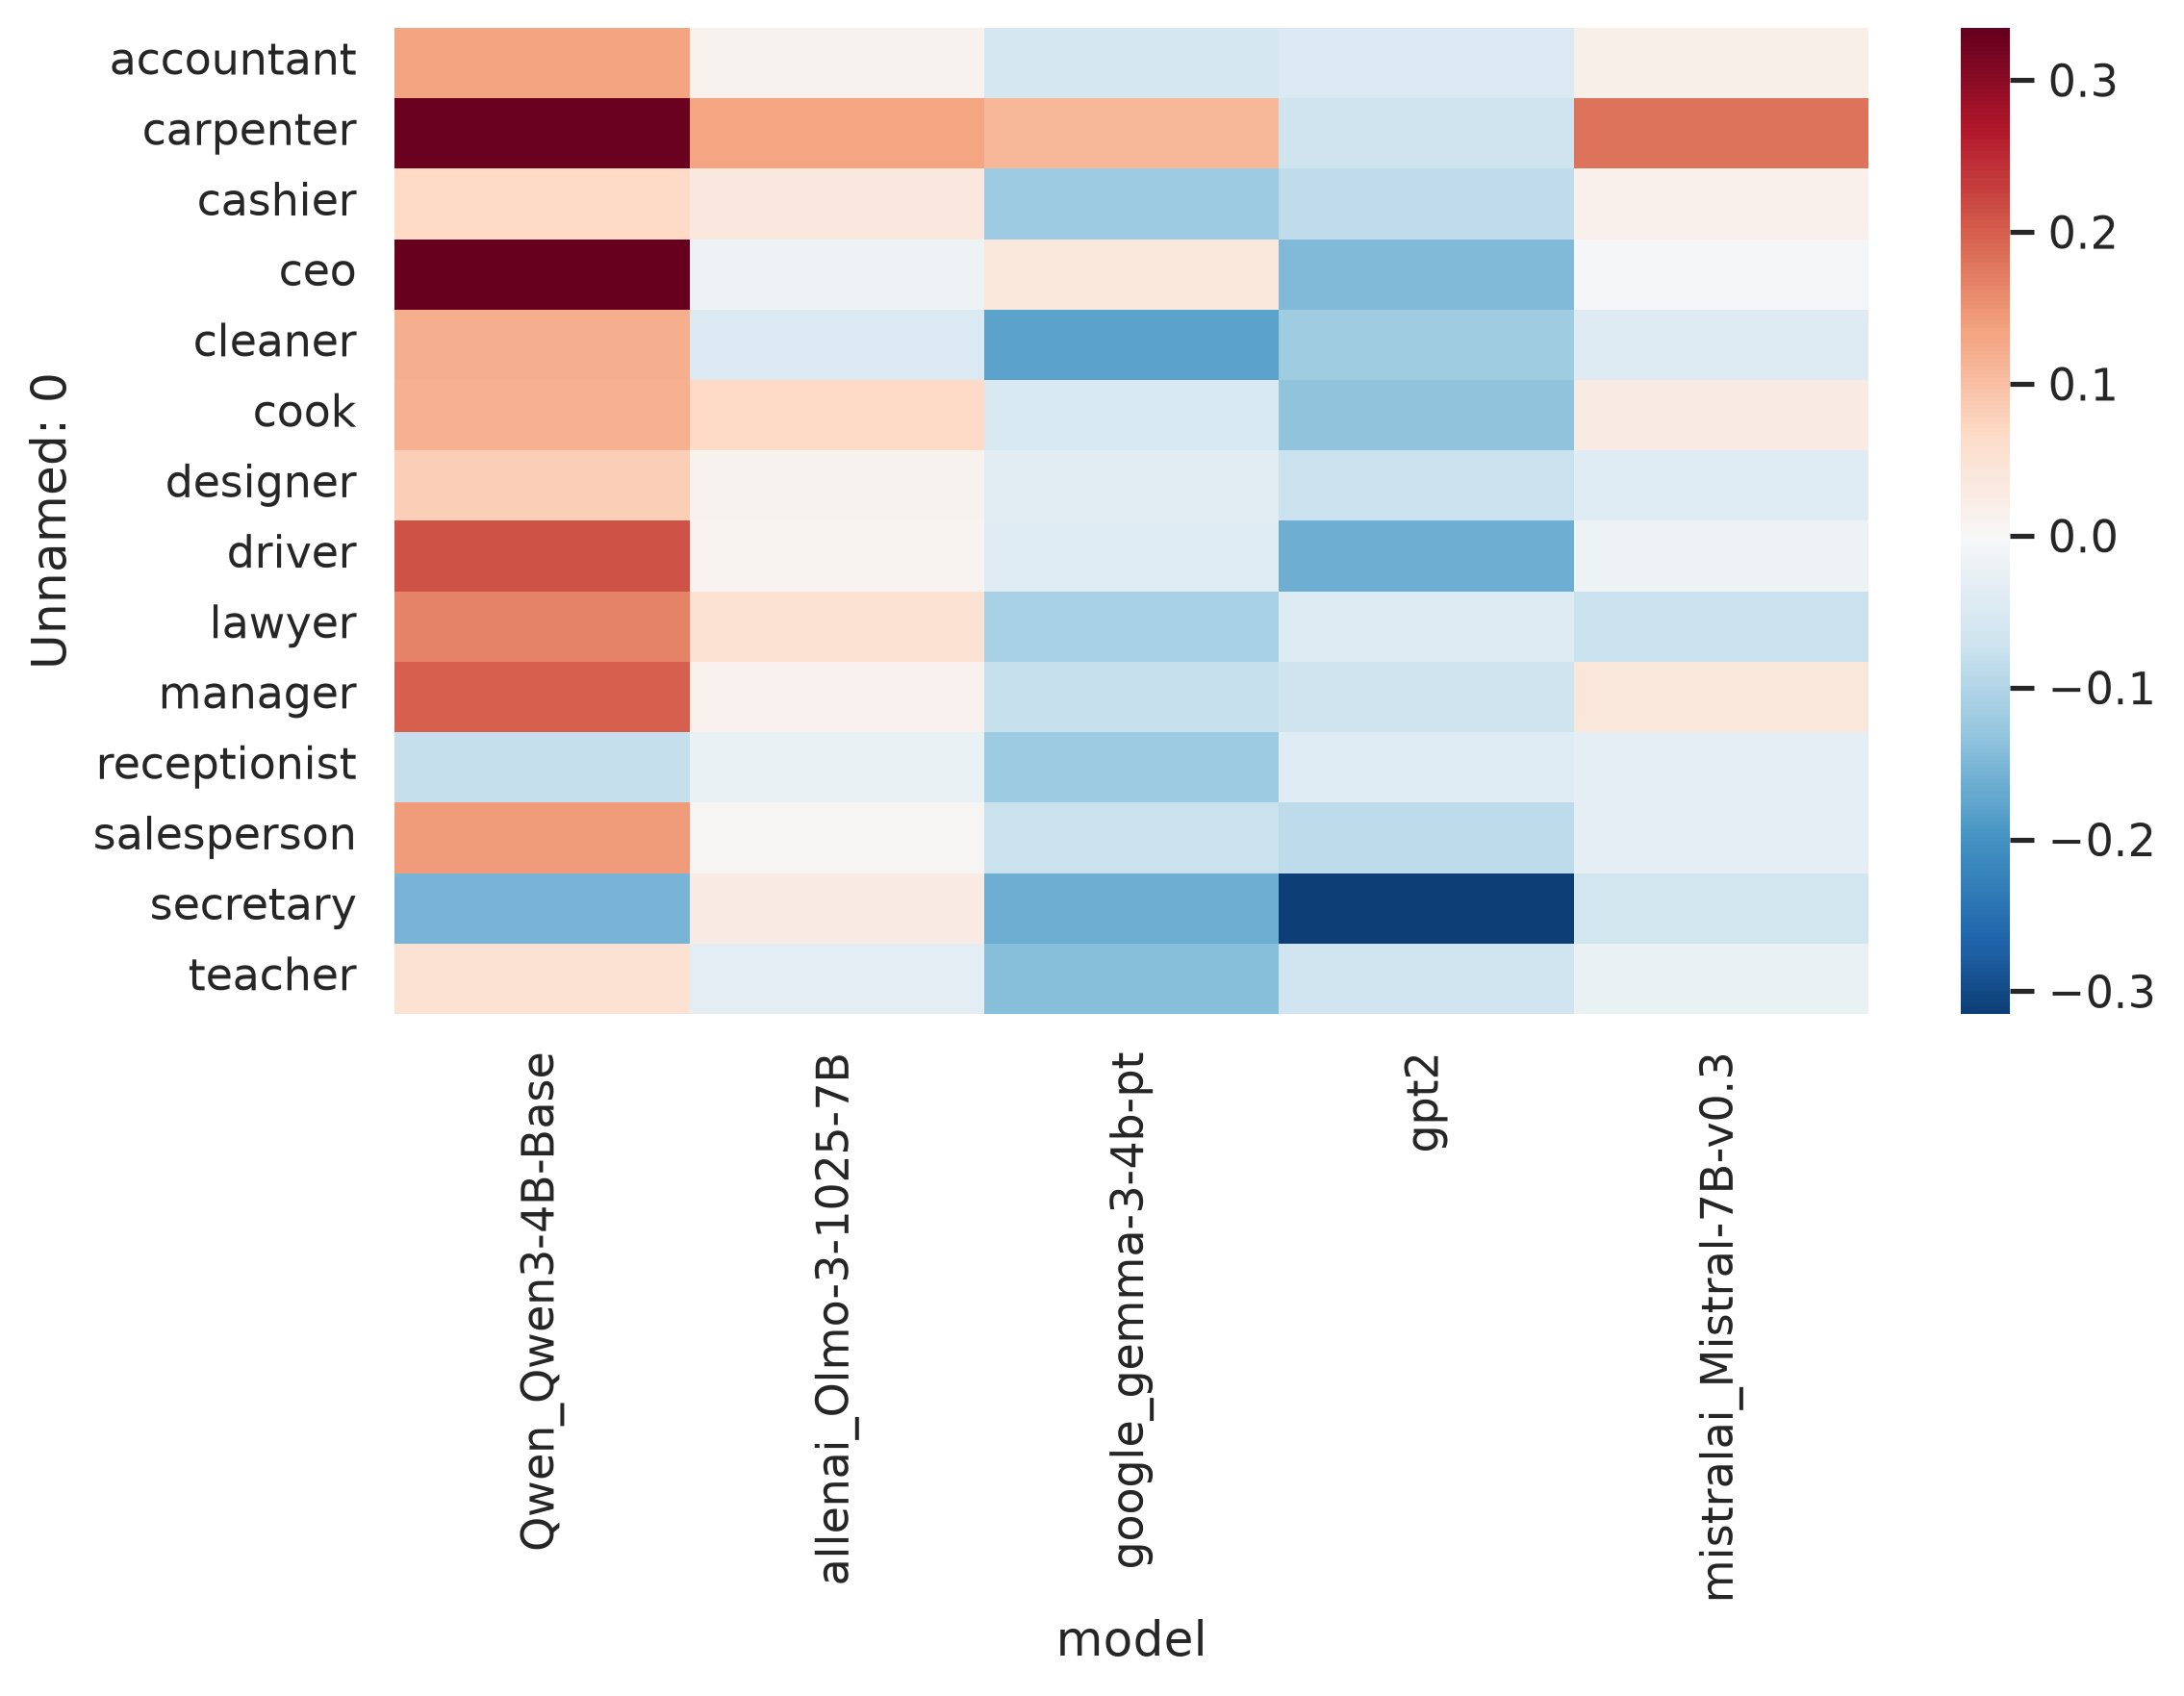
\includegraphics[width=.9\textwidth]{figures/profession_semantic_role_heatmap.png}
\caption{Semantic-role random effects.}
\end{figure}

\section{Cross-Model Similarity}

\begin{figure}[H]
\centering
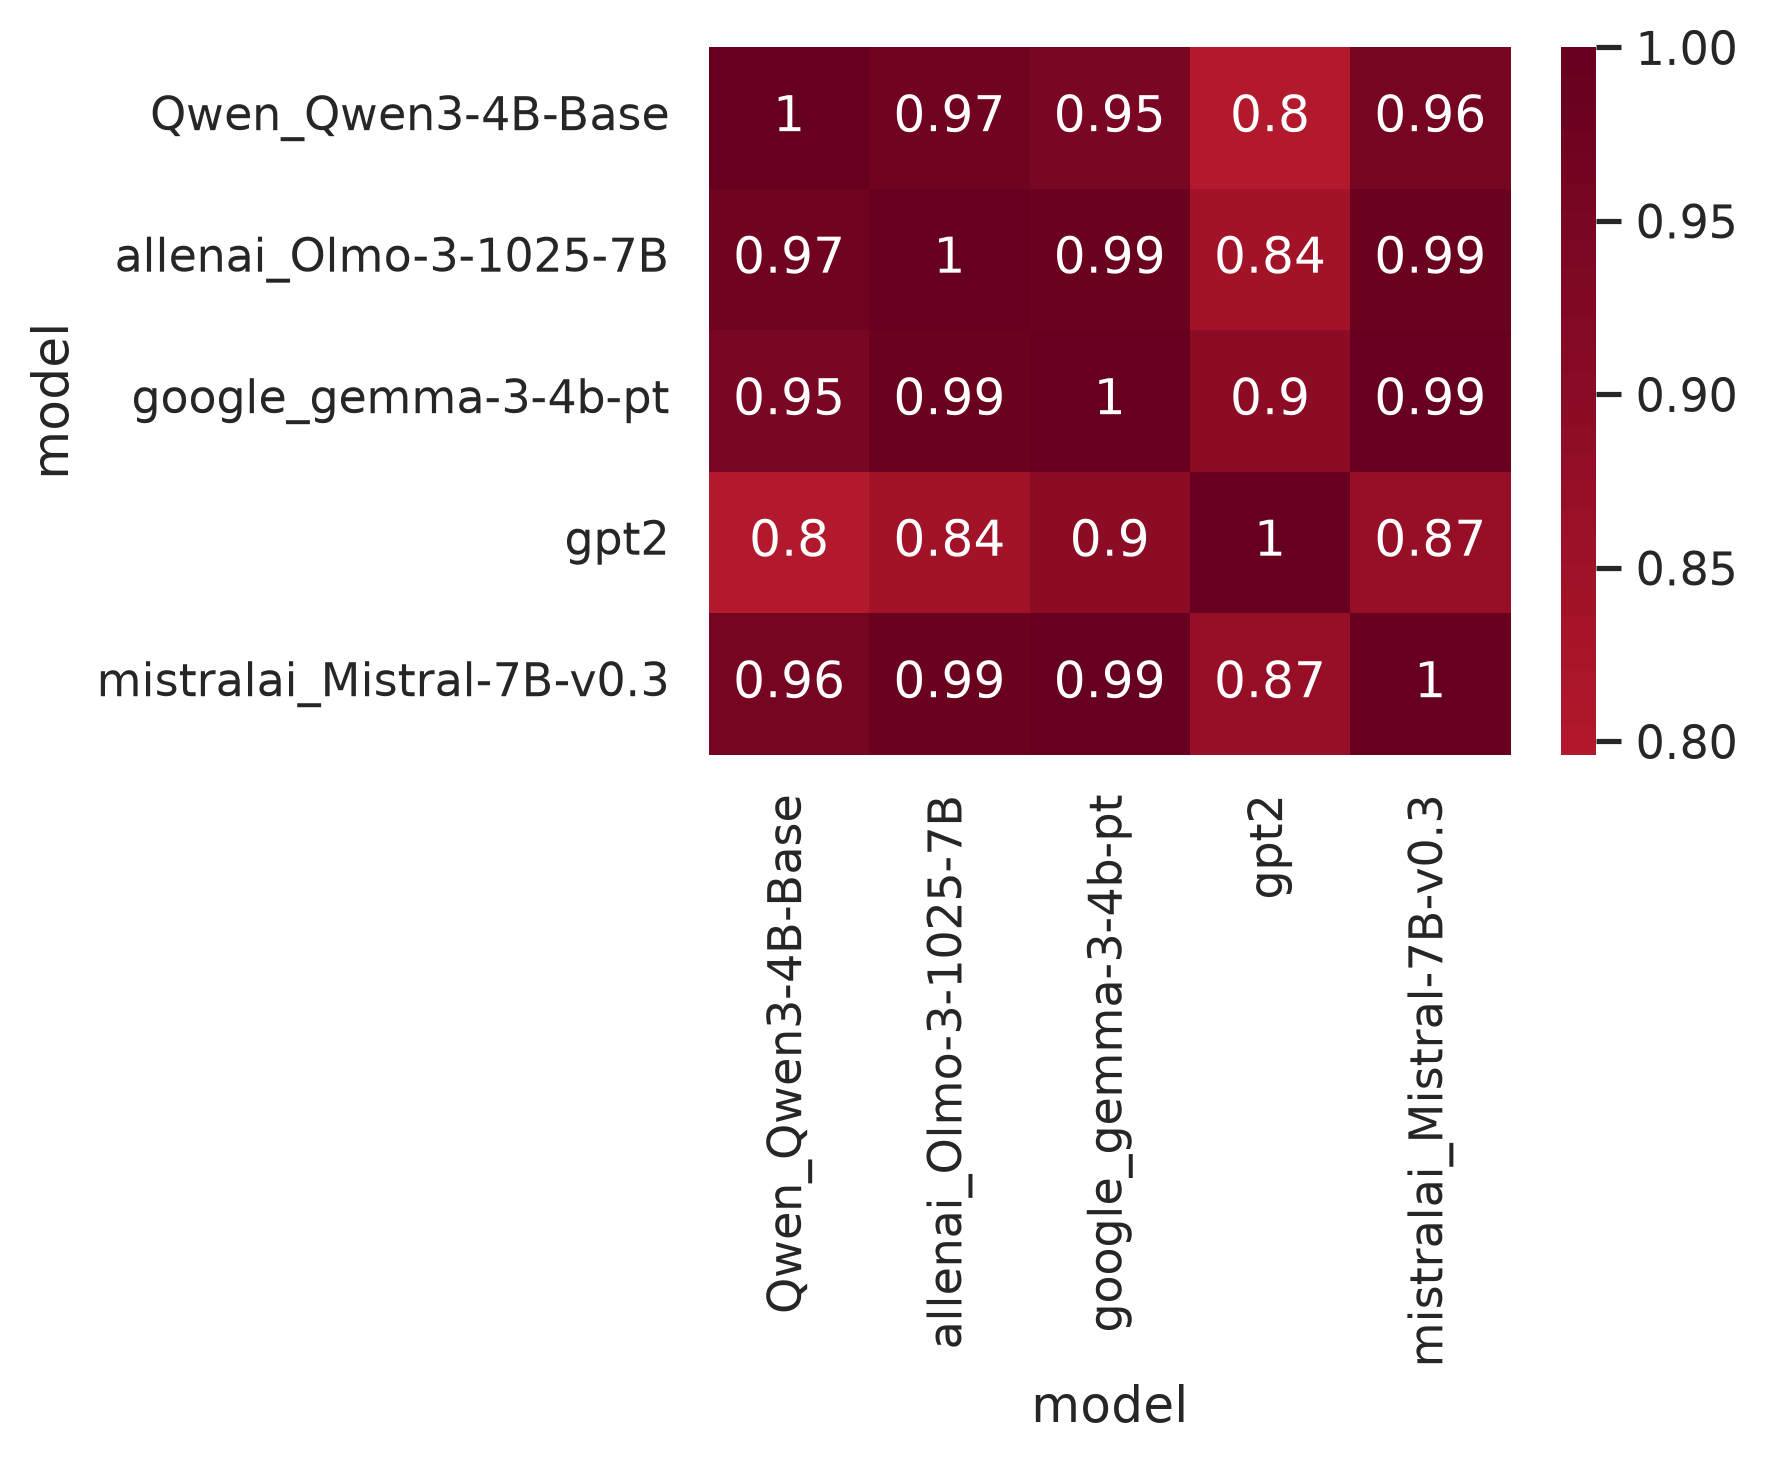
\includegraphics[width=.65\textwidth]{figures/intercept_correlation_matrix.png}
\caption{Correlation of profession intercepts.}
\end{figure}

\begin{figure}[H]
\centering
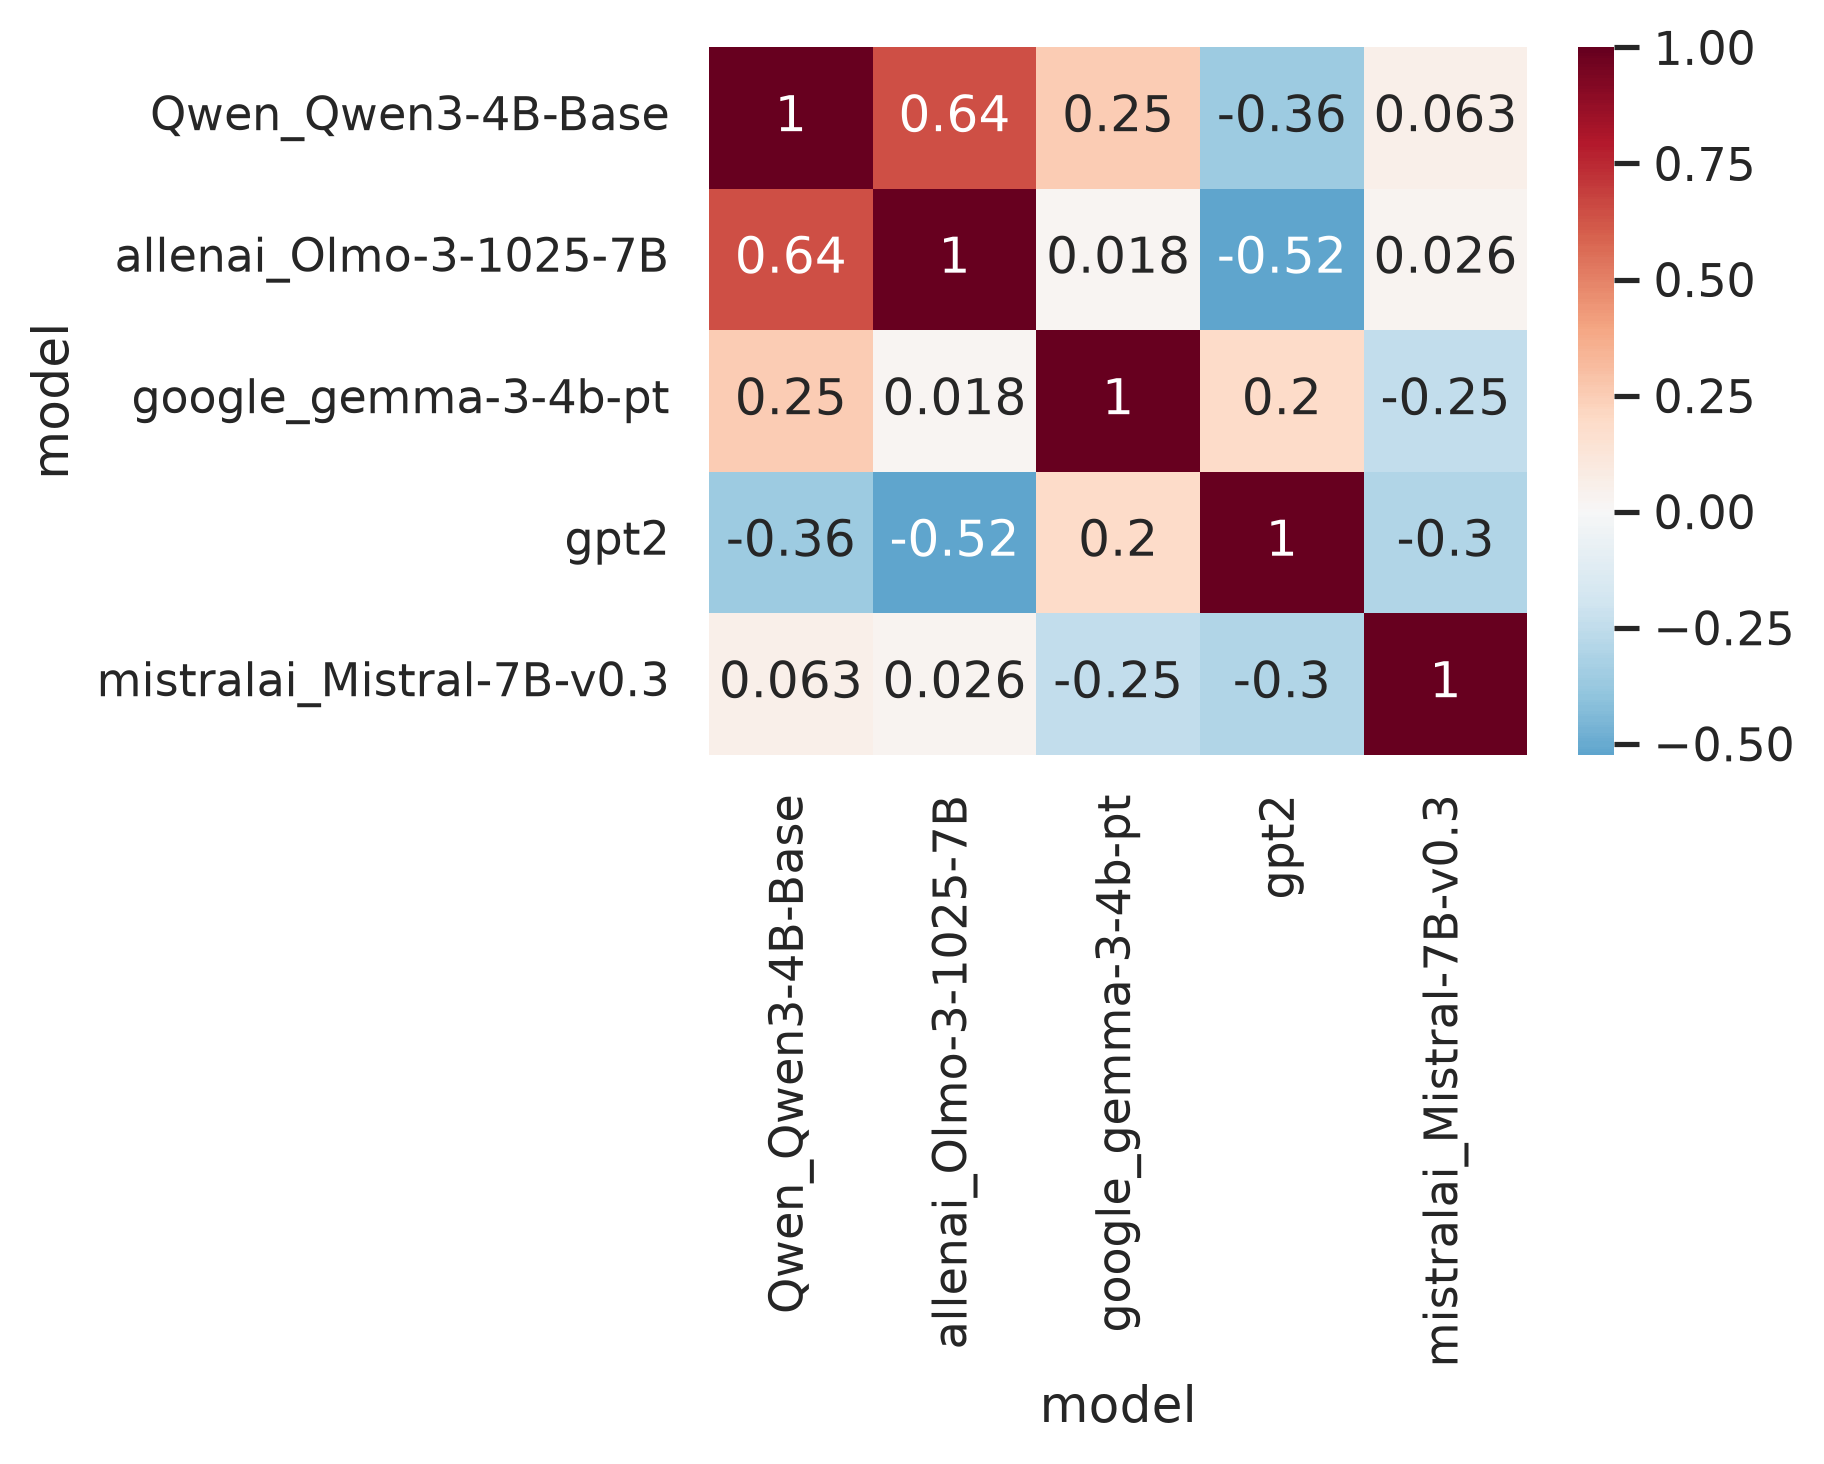
\includegraphics[width=.65\textwidth]{figures/syntactic_role_correlation_matrix.png}
\caption{Correlation of profession-specific syntactic-role effects.}
\end{figure}

\section{Profession PCA}

\begin{figure}[H]
\centering

\includegraphics[width=.8\textwidth]{figures/profession_pca.png}
\caption{PCA of profession random effects.}
\end{figure}

\section{Extreme Professions}

\begin{tabular}{llrlr}
\toprule
Model & HighestInterceptProfession & HighestIntercept & LowestInterceptProfession & LowestIntercept \\
\midrule
Qwen_Qwen3-4B-Base & carpenter & 2.547 & secretary & -0.930 \\
allenai_Olmo-3-1025-7B & carpenter & 2.775 & secretary & -1.609 \\
google_gemma-3-4b-pt & carpenter & 1.634 & receptionist & -2.596 \\
gpt2 & carpenter & 1.900 & receptionist & -1.703 \\
mistralai_Mistral-7B-v0.3 & carpenter & 2.273 & receptionist & -2.088 \\
\bottomrule
\end{tabular}


\section{Fixed Effects}

\begin{tabular}{lrrrrr}
\toprule
model & Qwen_Qwen3-4B-Base & allenai_Olmo-3-1025-7B & google_gemma-3-4b-pt & gpt2 & mistralai_Mistral-7B-v0.3 \\
\midrule
best_model_aic & 7355.178 & 6969.468 & 4523.552 & 2096.731 & 5524.240 \\
coef & 0.004 & 0.061 & 0.073 & 0.041 & 0.076 \\
std_err & 0.041 & 0.045 & 0.039 & 0.037 & 0.038 \\
p_value & 0.116 & 0.214 & 0.165 & 0.147 & 0.069 \\
ci_low & -0.076 & -0.026 & -0.004 & -0.032 & 0.001 \\
ci_high & 0.085 & 0.149 & 0.149 & 0.113 & 0.151 \\
random_effect_variance_semantic_role & 0.030 & 0.003 & 0.012 & 0.016 & 0.004 \\
random_effect_variance_syntactic_role & 0.088 & 0.030 & 0.019 & 0.028 & 0.007 \\
random_effect_variance_valence & 0.007 & 0.016 & 0.006 & 0.004 & 0.011 \\
random_effect_variance_dominance & 0.016 & 0.014 & 0.004 & 0.006 & 0.006 \\
\bottomrule
\end{tabular}


\begin{figure}[H]
\centering

\includegraphics[width=.95\textwidth]{figures/coefficient_heatmap.png}
\caption{Cross-model fixed-effect comparison.}
\end{figure}

\end{document}
